%==============================================================================
% 六、问题一的模型建立与求解
%==============================================================================
\section{问题一：感官评分的预测与分级}

\subsection{建模思路}

问题一要把 231 个化学指标映射到 50 个感官项的强度值。建模前先核实三件事，它们决定了模型的选择。

第一，输出不是整数等级。附件4 的 50 个感官项取值在 $-2.151$ 到 $6.172$ 之间，六成是负数，每一列的不同取值少则 106 个、多则 250 个。这说明它是中心化后的连续强度，不是 0--6 的评分。把取值平移到非负再四舍五入，中位 53.2\% 的样本会被压到 0 分，等级信息几乎全部丢失。因此本问按\emph{连续值回归}建模，等级放到最后用分位映射单独解决。

第二，样本量与特征数几乎相等。250 款酒对 231 个指标，比值接近 1。这种规模下任何模型都能把训练集拟合到 $R^2>0.9$，报出的精度若不与选择过程隔离，就只是挑选的结果。本文采用\emph{外层 5 折评估、内层 5 折选模型}的嵌套交叉验证，组织方式见 6.3 节。

第三，目标之间难度差异极大。同一数据集的原论文\cite{schreurs2024}报告梯度提升在训练感官面板上的多输出 $R^2$ 约为 0.21，本文以此为参照上限：结果远低于它说明实现有问题，接近它则说明这是数据本身的信息量边界。

基于这三点，本问取四个回归模型并列比较，每个感官项各自取内层最优，而不预先指定其中任何一个。

\begin{itemize}
  \item \textbf{岭回归}：线性模型加 $\ell_2$ 惩罚，把系数整体压小，适合处理共线，但抓不住非线性。
  \item \textbf{弹性网}：线性模型同时加 $\ell_1$ 与 $\ell_2$ 惩罚，既压系数又做变量筛选，输出比岭回归稀疏、更易解释。
  \item \textbf{LightGBM}：梯度提升树，逐轮拟合前一轮的残差，按直方图选分裂点，能刻画非线性与特征交互。
  \item \textbf{ExtraTrees}：极端随机树，在随机切分点上建大量树后取平均，方差远低于单棵树，在 250 个样本上更稳。
\end{itemize}

此外，50 项里有 9 项的地板效应占比超过 0.30，即三成以上样本挤在该项最低值附近，barnyard 达 0.476。这类项用普通回归会把“没有感知到”与“感知到但很弱”混为同一件事。对它们本文改用\emph{两段式模型}：先用梯度提升分类器判断该项是否被感知，再用回归器在已感知样本上估计强度，两者相乘。被划入两段式的是 acetic、lactic、coriander、A\_malt\_burn、orange、clove、barnyard、F\_hops\_tropical、stale\_hops 共 9 项，以酸味、香料与缺陷味为主。

\subsection{模型建立}

设第 $i$ 个样本的化学特征为 $\boldsymbol{x}_i\in\mathbb{R}^{231}$，第 $s$ 个感官项的强度为 $y_{is}$。四个模型中，岭回归与弹性网有显式目标函数，树模型没有。

岭回归最小化残差平方和加 $\ell_2$ 惩罚
\begin{equation}
  \hat{\boldsymbol\beta}^{\mathrm{ridge}}_s=\arg\min_{\boldsymbol\beta}\ \frac{1}{2N}\lVert \boldsymbol{y}_s-\boldsymbol{X}\boldsymbol\beta\rVert_2^2+\lambda\lVert\boldsymbol\beta\rVert_2^2 .
\end{equation}
弹性网在惩罚项里再加一个 $\ell_1$ 分量
\begin{equation}
  \hat{\boldsymbol\beta}^{\mathrm{enet}}_s=\arg\min_{\boldsymbol\beta}\ \frac{1}{2N}\lVert \boldsymbol{y}_s-\boldsymbol{X}\boldsymbol\beta\rVert_2^2
  +\lambda\left(\alpha\lVert\boldsymbol\beta\rVert_1+\frac{1-\alpha}{2}\lVert\boldsymbol\beta\rVert_2^2\right),
\end{equation}
其中 $\lambda$ 与 $\alpha$ 都在内层交叉验证上选。LightGBM 与 ExtraTrees 不写目标函数：前者以均方误差为损失逐轮拟合负梯度，后者对每个节点在随机阈值上切分、对多棵树取算术平均。

两段式模型的预测值是两个阶段的加权混合，而非相乘
\begin{equation}
  \hat y_{is}=\left(1-\hat\pi_{is}\right)\bar y_s^{\text{floor}}+\hat\pi_{is}\,\hat\mu_{is},\qquad
  \hat\pi_{is}=\Pr\left(y_{is}>y_s^{\min}\mid \boldsymbol{x}_i\right),
\end{equation}
其中 $\hat\pi_{is}$ 由梯度提升分类器给出，$\hat\mu_{is}$ 由回归器在 $y_{is}>y_s^{\min}$ 的样本上给出，$\bar y_s^{\text{floor}}$ 为左尾样本（$y\le y_s^{\min}+0.15$）的强度均值。此处不用 $\hat\pi\hat\mu$ 的乘积形式，是因为乘积会把左尾样本的预测强行拉到 0，而实测中这类样本的强度并不为 0（只是集中在列最小值附近），相乘会系统性低估其强度；加权混合保留了“落在左尾时取左尾均值”这一含义，也让 $\hat\pi$ 退化为 0/1 时连续过渡到单段回归。需要说明的是，这里的 $\hat\pi$ 是“强度高于左尾窗”的概率，不是“是否感知到”的概率——附件4 的标签已按品评员做过 z-score，负值代表低于该品评员的平均，不代表没有尝到（见 5.3 节）。

评价用决定系数与平均绝对误差
\begin{equation}
  R^2_s=1-\frac{\sum_i\left(y_{is}-\hat y_{is}\right)^2}{\sum_i\left(y_{is}-\bar y_s\right)^2},
  \qquad
  \mathrm{MAE}_s=\frac{1}{n}\sum_i\left|y_{is}-\hat y_{is}\right|,
\end{equation}
并用 1000 次自助重采样在折外预测上给出 $R^2$ 的 95\% 置信区间。

\subsection{模型求解}

\noindent\textbf{交叉验证的组织方式}\quad 普通 5 折交叉验证的缺陷在于，选模型的数据与报分数的数据是同一批，四个模型里挑最好的那个，报出的分数就已经带上了挑选的痕迹；模型越多、特征越多，这种乐观偏差越大。本问有 250 个样本、231 个特征，若用普通 5 折，报出的 $R^2$ 会系统性偏高。

嵌套交叉验证把它拆成两层。外层 5 折只做一件事：把 250 个样本切成训练集 200 个与评估集 50 个。内层 5 折在训练集的 200 个样本内部再切一次，用内层 5 折的折外预测算出四个模型各自的 $R^2$，取最高的那个作为本折的选定模型。选定之后，用这 200 个样本全量重训该模型，再预测被留出的 50 个样本。评估集从头到尾不参与任何选择，因此报出的数才是泛化误差的无偏估计。代价是训练次数乘 5。

\noindent\textbf{四个模型的具体设置}\quad 四个模型的超参在建模前固定，不在交叉验证里搜索。这样做有两个考虑：一是 250 个样本上做超参网格，搜出来的最优值本身不稳定，反而增加选择偏差；二是固定超参后，四个模型之间的差异只来自模型族本身，比较结果更干净。具体取值见表~\ref{tab:q1hyper}。

\begin{table}[htbp]
\centering
\footnotesize
\caption{问题一四个候选模型的超参设置，建模前固定，不在交叉验证内搜索}
\label{tab:q1hyper}
\begin{tabular*}{\textwidth}{@{\extracolsep{\fill}}llp{7.4cm}@{}}
\toprule
\textbf{模型} & \textbf{类型} & \textbf{超参取值} \\
\midrule
岭回归 & 线性，$\ell_2$ 正则 & $\alpha=10$ \\
弹性网 & 线性，$\ell_1+\ell_2$ 正则 & $\alpha=0.05$，$\ell_1$ 比例 $0.5$，最大迭代 5000 \\
LightGBM & 梯度提升树 & 150 棵树，叶数 7，最小叶样本 8，学习率 0.06，行采样 0.8，列采样 0.6，$\ell_2$ 惩罚 1.0 \\
ExtraTrees & 极端随机树 & 200 棵树，每节点随机特征数 $\sqrt{p}$，最小叶样本 3 \\
\bottomrule
\end{tabular*}
\end{table}

标准化在每一折内部单独做：用训练折的中位数填补缺失、用训练折的均值与标准差做标准化，再把同一套参数用到评估折。若改用全表均值填补，评估折的信息就会提前泄露进训练。

两段式模型只在 9 个左尾占比超过 0.30 的感官项上启用，其分类头与回归头分别取与表中四个模型对应的组合，例如 LightGBM 分类配 LightGBM 回归、逻辑回归配岭回归，同样在内层 5 折里择优。

\noindent\textbf{实际计算量}\quad 按上述组织，全部计算量为外层 5 折、50 个感官项、4 个模型与内层 5 折的乘积，再加 50 次全量重训，共 5250 次模型拟合；两段式项每次拟合含分类与回归两个头，折算后实际拟合约 6100 次。区间估计在折外预测上做 1000 次自助重采样，每个感官项 1000 次、共 5 万次重采样，这一步只做排序与分位数计算，不再重训模型。

随机种子统一取 2026，树的并行度设为 4 进程，全部 50 项在单机串行跑完，耗时 273.6 秒，可作为复现的基准。

\subsection{结果分析：总体精度}

50 项的嵌套交叉验证结果为：$R^2$ 中位 0.1469、均值 0.2223；49 项为正，14 项超过 0.3、6 项超过 0.5、19 项低于 0.10；32 项的自助区间下界大于 0。区间宽度中位 0.1936，远大于 1000 次重采样的蒙特卡洛噪声，约 0.006，说明区间本身是稳的。图~\ref{fig:q1forest} 给出逐项的 $R^2$ 与区间，按数值排序。

\begin{figure}[htbp]
\centering
\begin{subfigure}[t]{0.48\textwidth}
\centering
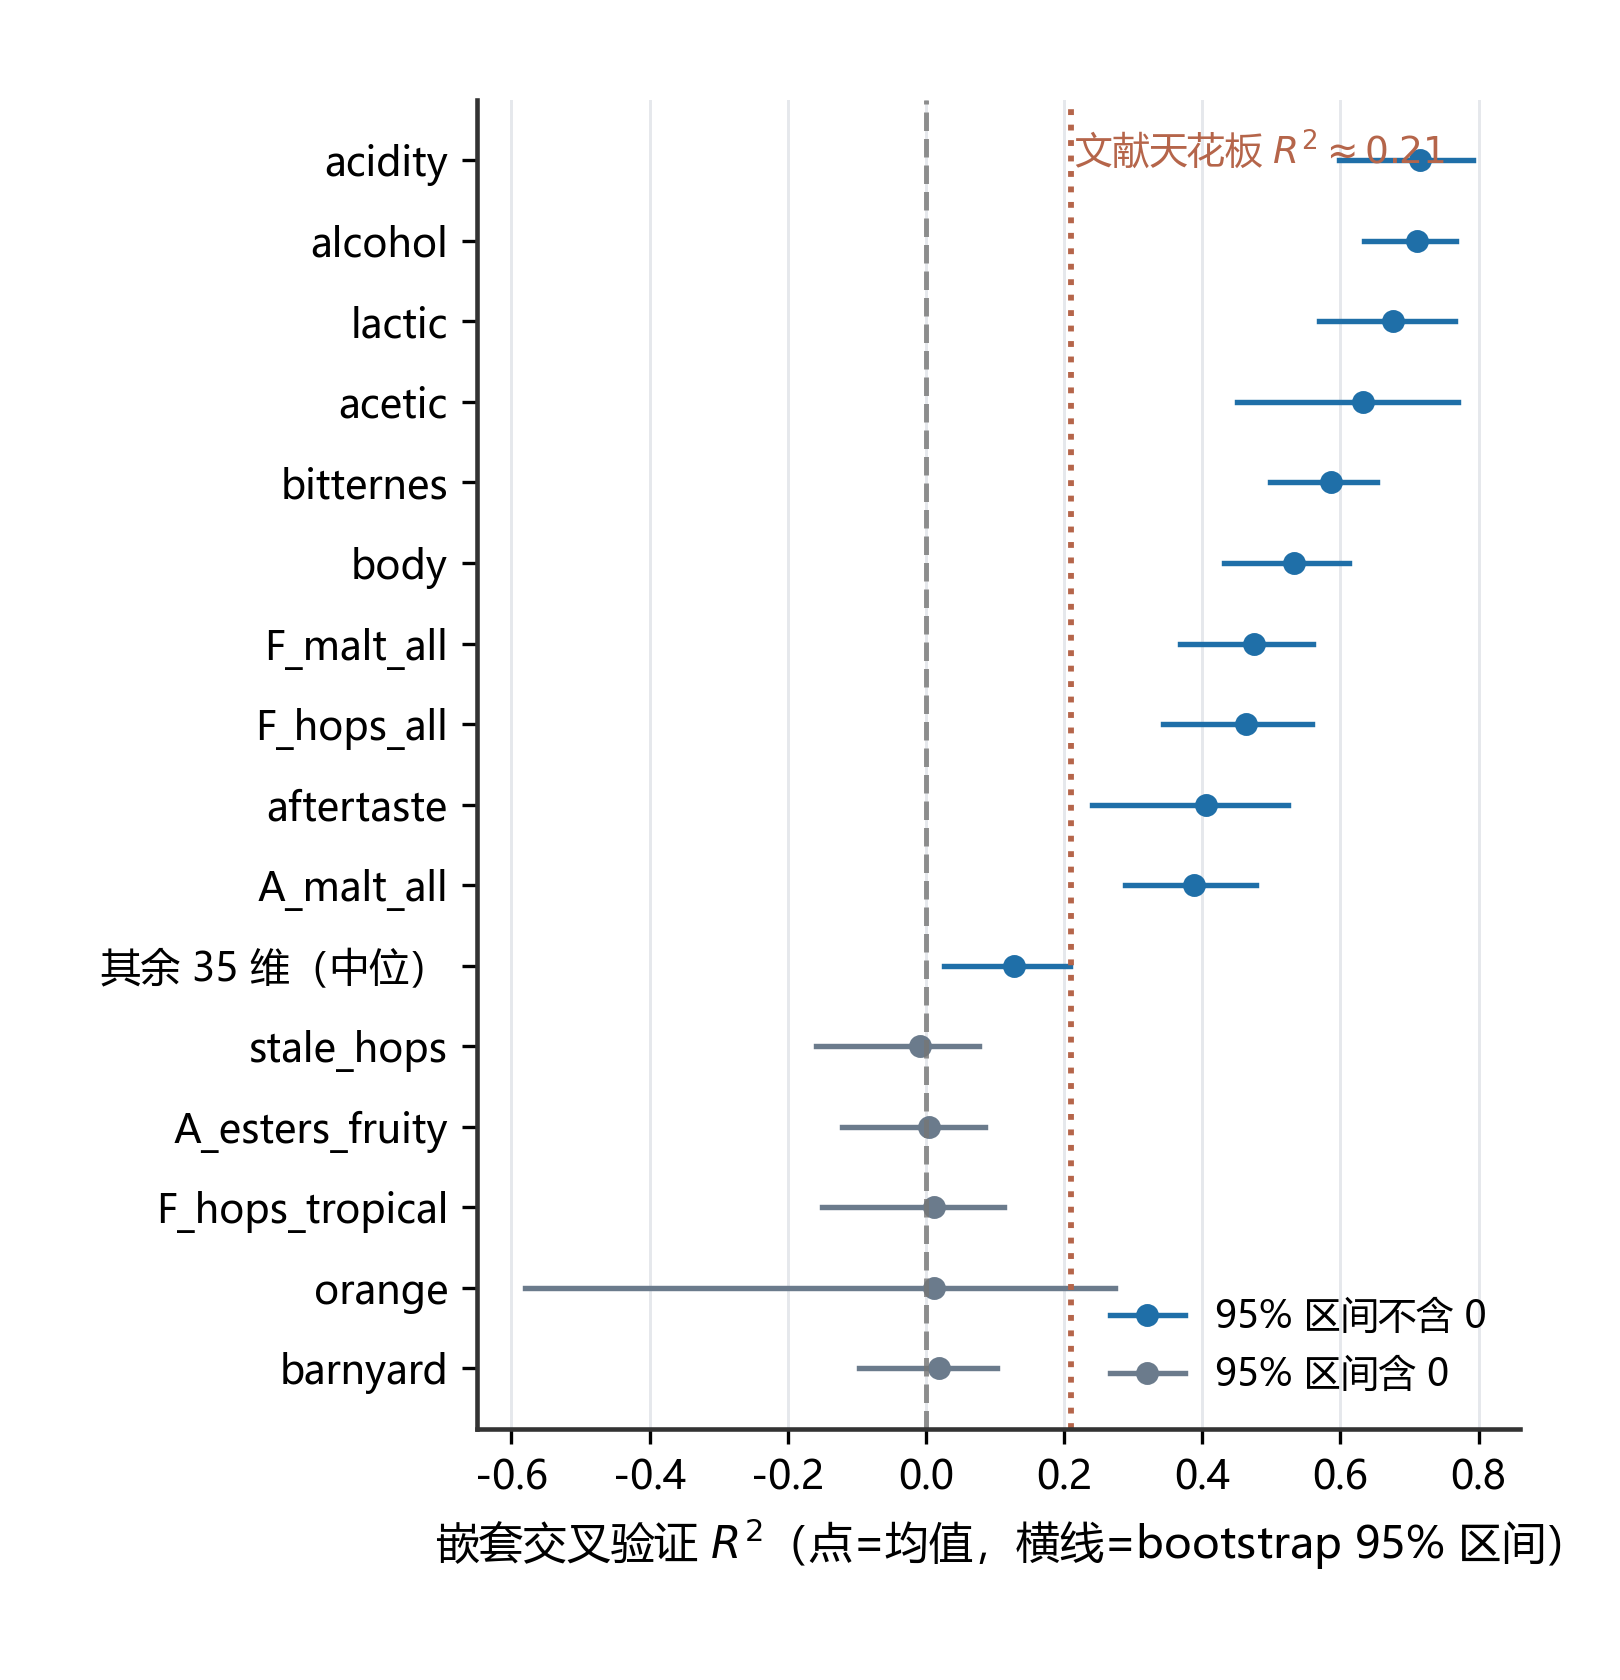
\includegraphics[width=\linewidth]{figures/fig_q1_r2_forest.png}
\caption{50 个感官项的 $R^2$ 与自助 95\% 区间。蓝点表示区间不含 0，灰点表示区间含 0}
\label{fig:q1forest}
\end{subfigure}
\hfill
\begin{subfigure}[t]{0.48\textwidth}
\centering
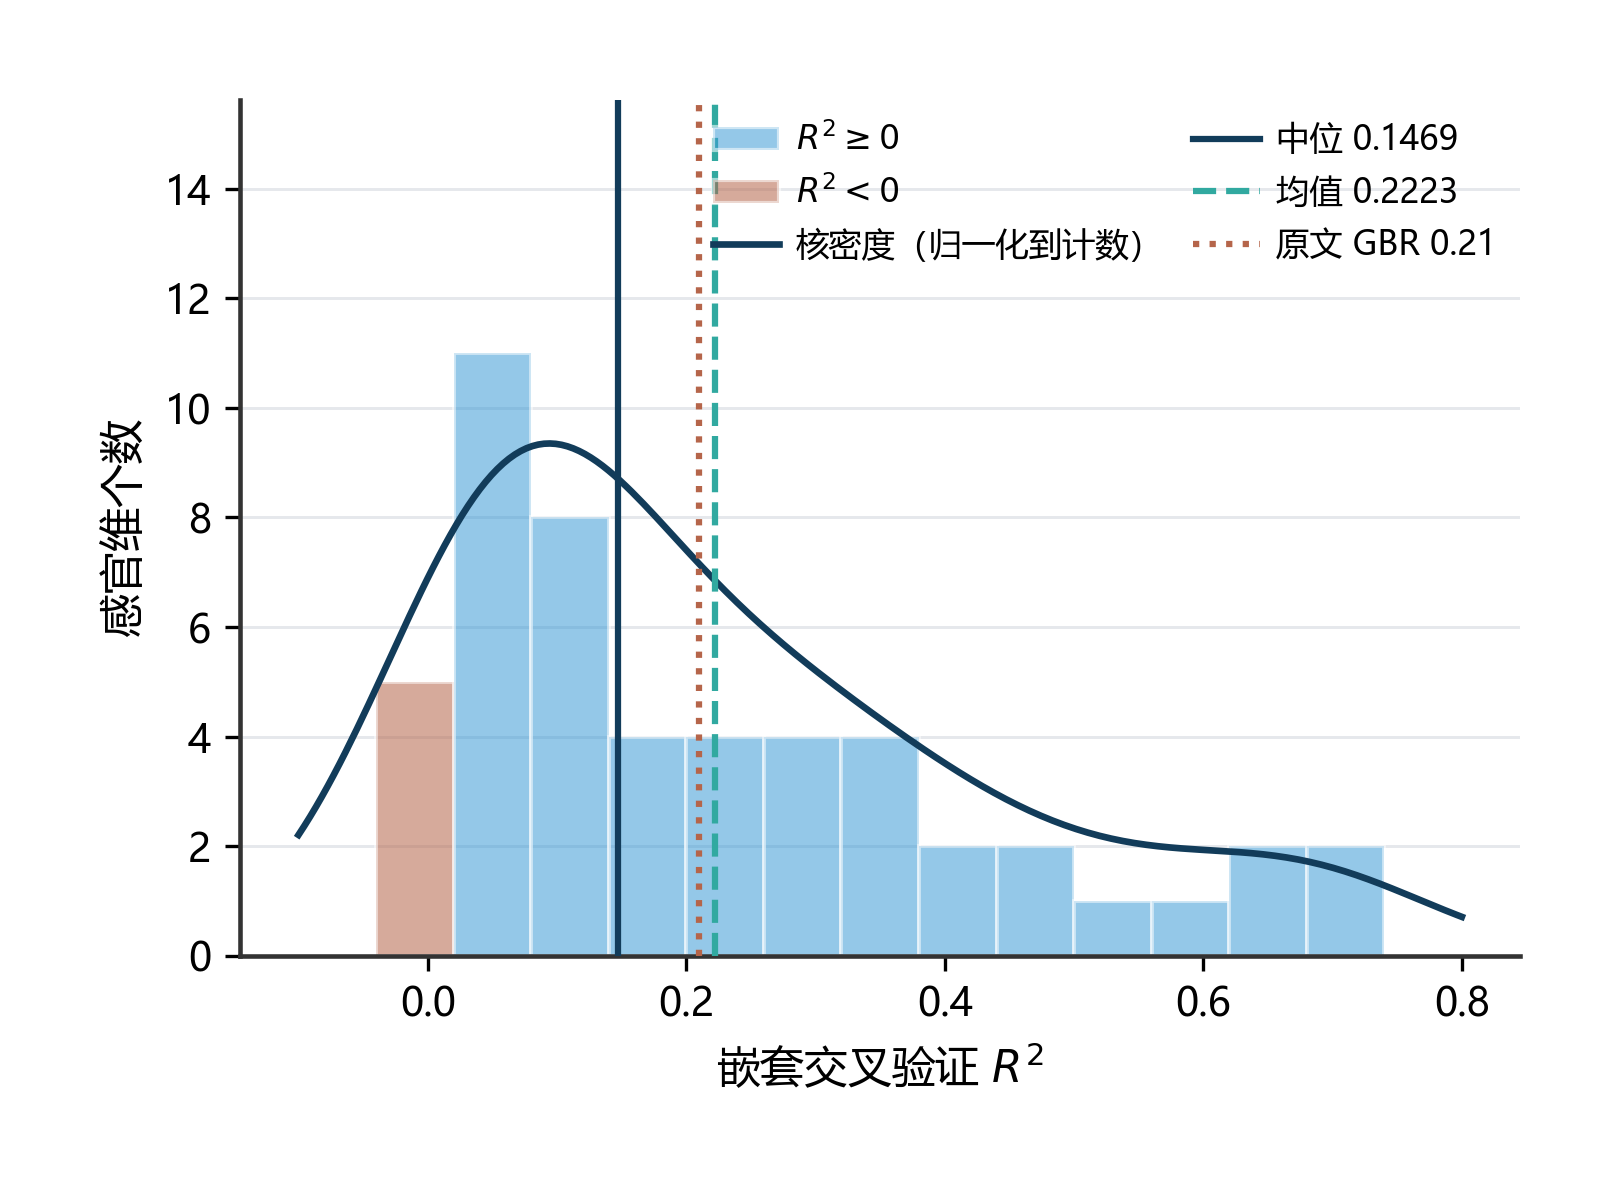
\includegraphics[width=\linewidth]{figures/fig_q1_r2_dist.png}
\caption{$R^2$ 的分布，竖线为中位数、均值与文献报道的梯度提升水平}
\label{fig:q1dist}
\end{subfigure}
\caption{问题一的 $R^2$ 结果。左图为 50 个感官项的 $R^2$ 与自助 95\% 区间，蓝点为区间不含 0；右图为 $R^2$ 的分布，三条竖线分别是中位数 0.1469、均值 0.2223 与文献报道的梯度提升水平 0.21}
\end{figure}

\subsection{结果分析：逐项结果与模型分工}

逐项看是散点，整体看是分布。图~\ref{fig:q1dist} 把 50 个 $R^2$ 叠成一张直方图并叠加核密度，三条竖线分别是中位数 0.1469、均值 0.2223 与文献\cite{schreurs2024}报道的梯度提升水平 0.21。中位比均值低 0.0754 是右偏的直接证据：多数项挤在 0.10 到 0.20 之间，少数理化直连的项把均值拉了上去，其中酸度 0.7149、酒精 0.7108、乙酸 0.6326、乳酸 0.6768。均值 0.2223 与文献的 0.21 几乎重合，说明整体信息量没有被浪费；而中位偏低说明这个均值是靠少数项撑起来的，不代表普遍水平。



四个模型被选中的次数说明了各自的分工：ExtraTrees 24 次、LightGBM 20 次、弹性网 6 次、岭回归一次也没有胜出。这个分布与 5.3 节测到的共线结构吻合——219 列的方差膨胀因子大于 10 时，纯岭惩罚压不住系数，树模型靠分裂绕开了这个问题，而弹性网的 $\ell_1$ 分量能在 231 列里挑出少数有用的列，所以在 body、F\_malt\_all、A\_malt\_all 这类信号稀疏的项上胜出。

可预测性最高的是 acidity 与 alcohol,$R^2$ 分别为 0.7149 与 0.7108。这两项对应酸度与乙醇浓度的直接化学测量，机理清楚，模型学到的基本上是线性关系。表~\ref{tab:q1} 列出前 10 项，其中 acetic 与 lactic 的地板效应占比高达 0.61 与 0.69，是靠两段式模型才取得 0.63 与 0.61 的——若用单段回归，这两项会被“大量样本压在最低值”拖垮。

\begin{table}[htbp]
\centering
\footnotesize
\caption{问题一前 10 个感官项的嵌套交叉验证结果}
\label{tab:q1}
\begin{tabular*}{\textwidth}{@{\extracolsep{\fill}}lcccc}
\toprule
\textbf{感官项} & \textbf{选中模型} & $R^2$ & \textbf{95\% 区间} & \textbf{MAE} \\
\midrule
acidity & LightGBM & 0.7149 & $[0.598,\ 0.791]$ & 0.2995 \\
alcohol & LightGBM & 0.7108 & $[0.634,\ 0.767]$ & 0.3268 \\
acetic & LightGBM（两段式） & 0.6326 & $[0.450,\ 0.771]$ & 0.1934 \\
lactic & LightGBM（两段式） & 0.6768 & $[0.569,\ 0.767]$ & 0.1875 \\
bitternes & LightGBM & 0.5862 & $[0.498,\ 0.652]$ & 0.3693 \\
body & 弹性网 & 0.5328 & $[0.431,\ 0.613]$ & 0.3038 \\
F\_malt\_all & 弹性网 & 0.4750 & $[0.368,\ 0.560]$ & 0.4033 \\
F\_hops\_all & LightGBM & 0.4639 & $[0.344,\ 0.559]$ & 0.3975 \\
aftertaste & LightGBM & 0.4048 & $[0.240,\ 0.524]$ & 0.3597 \\
A\_malt\_all & 弹性网 & 0.3795 & $[0.278,\ 0.466]$ & 0.4414 \\
\bottomrule
\end{tabular*}
\end{table}

中位 0.1469 比文献报告的 0.21 低 0.06，但均值 0.2223 与文献持平。两个数一起看才有意义：均值持平说明整体信息量没有被浪费，中位偏低说明分布是右偏的——少数理化直连的项被解释得较好，多数香气项几乎不可解释。这不是实现问题，而是 250 个样本下各项信息量本身差异极大。

\subsection{结果分析：预测质量与残差诊断}

$R^2$ 只说明整体解释力，看不出误差是怎么分布的。预测质量比 $R^2$ 数字更直观。图~\ref{fig:q1reg} 用四项做对照：alcohol 与 acidity 的散点紧贴 $y=x$;bitternes 的秩相关仍有 0.74，但斜率明显小于 1，高苦度样本被系统性低估，这是折外预测向均值收缩的常见表现；F\_esters\_flower 的散点是一团水平云，$R^2$ 只有 0.0293，模型对这一项没有解释力。越是贴近对角线的项，其 Top-3 归因才越可信，这一点在第七章会用到。

\begin{figure}[htbp]
\centering
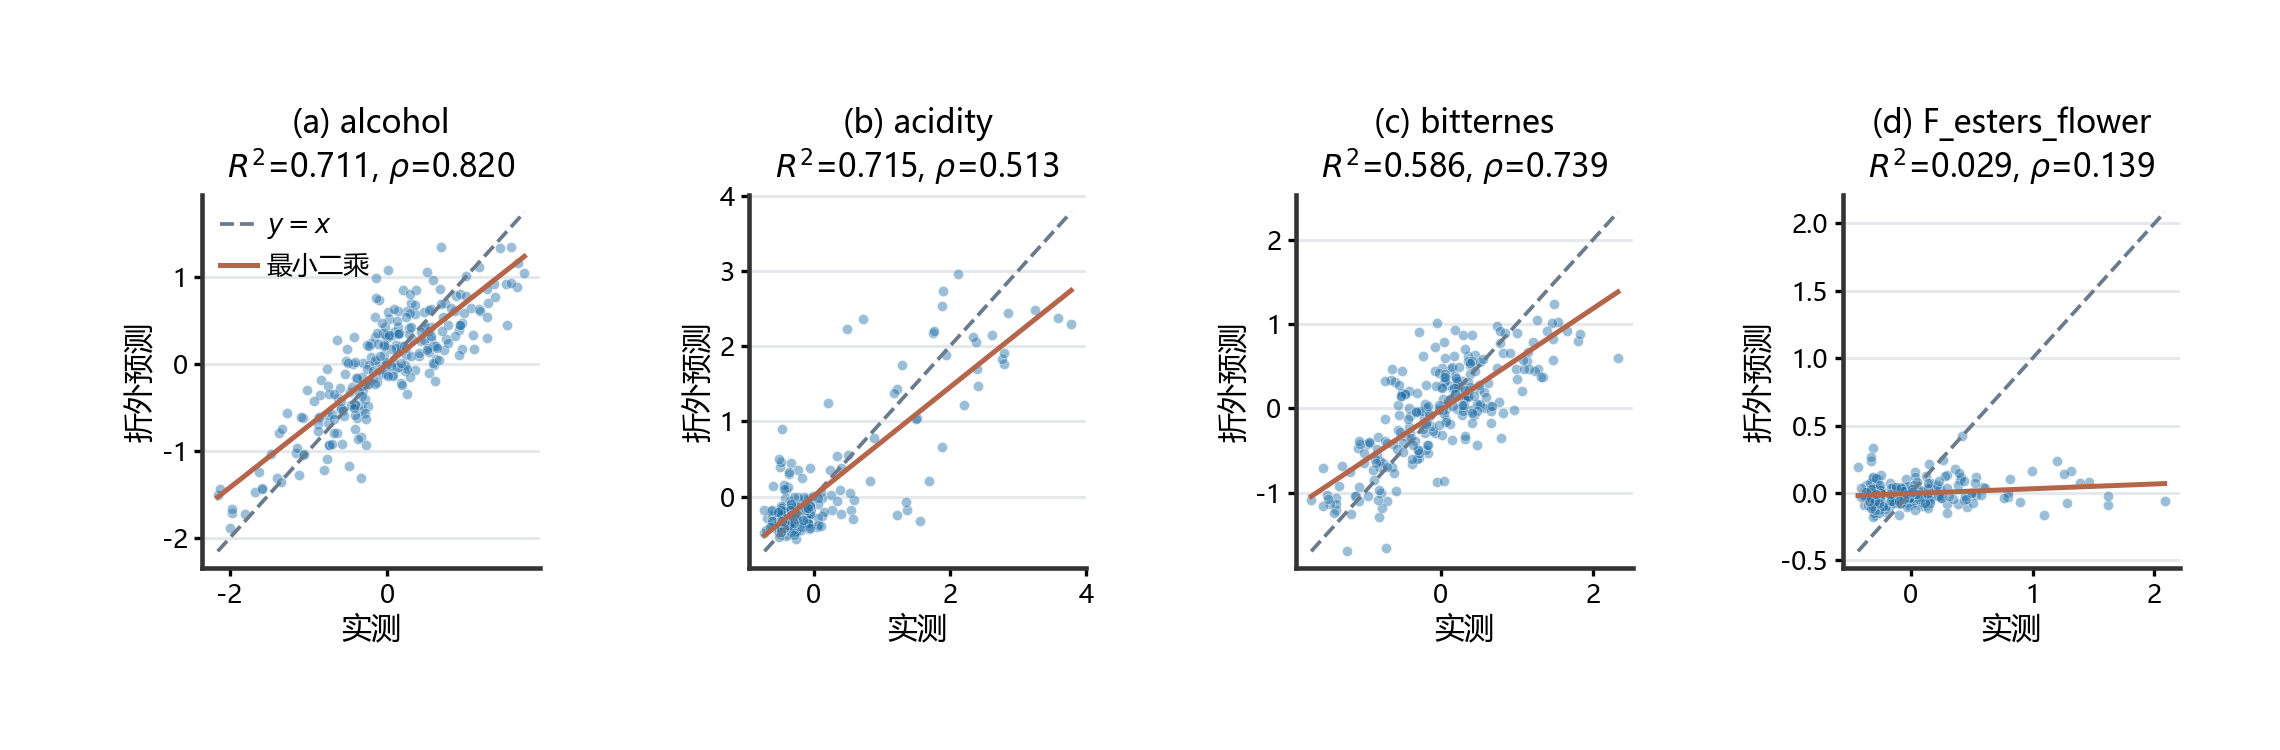
\includegraphics[width=0.86\textwidth]{figures/fig_q1_reg_fit.png}
\caption{四个代表性项的折外预测与实测对照：alcohol 与 acidity 紧贴对角线，bitternes 斜率偏小，F\_esters\_flower 呈水平云团}
\label{fig:q1reg}
\end{figure}

残差诊断进一步验证模型设定。图~\ref{fig:q1res} 对 alcohol 做四项检验：残差对拟合值没有漏斗形，同方差成立；偏度 0.055、Shapiro--Wilk 检验 $p=0.914$，不能拒绝正态；Q--Q 图贴合对角线，最大标准化残差 2.76，没有样本超过 3 倍标准差；残差对样本序号无趋势。四项都没有发现系统性偏差，说明该维的模型设定是恰当的。

\begin{figure}[htbp]
\centering
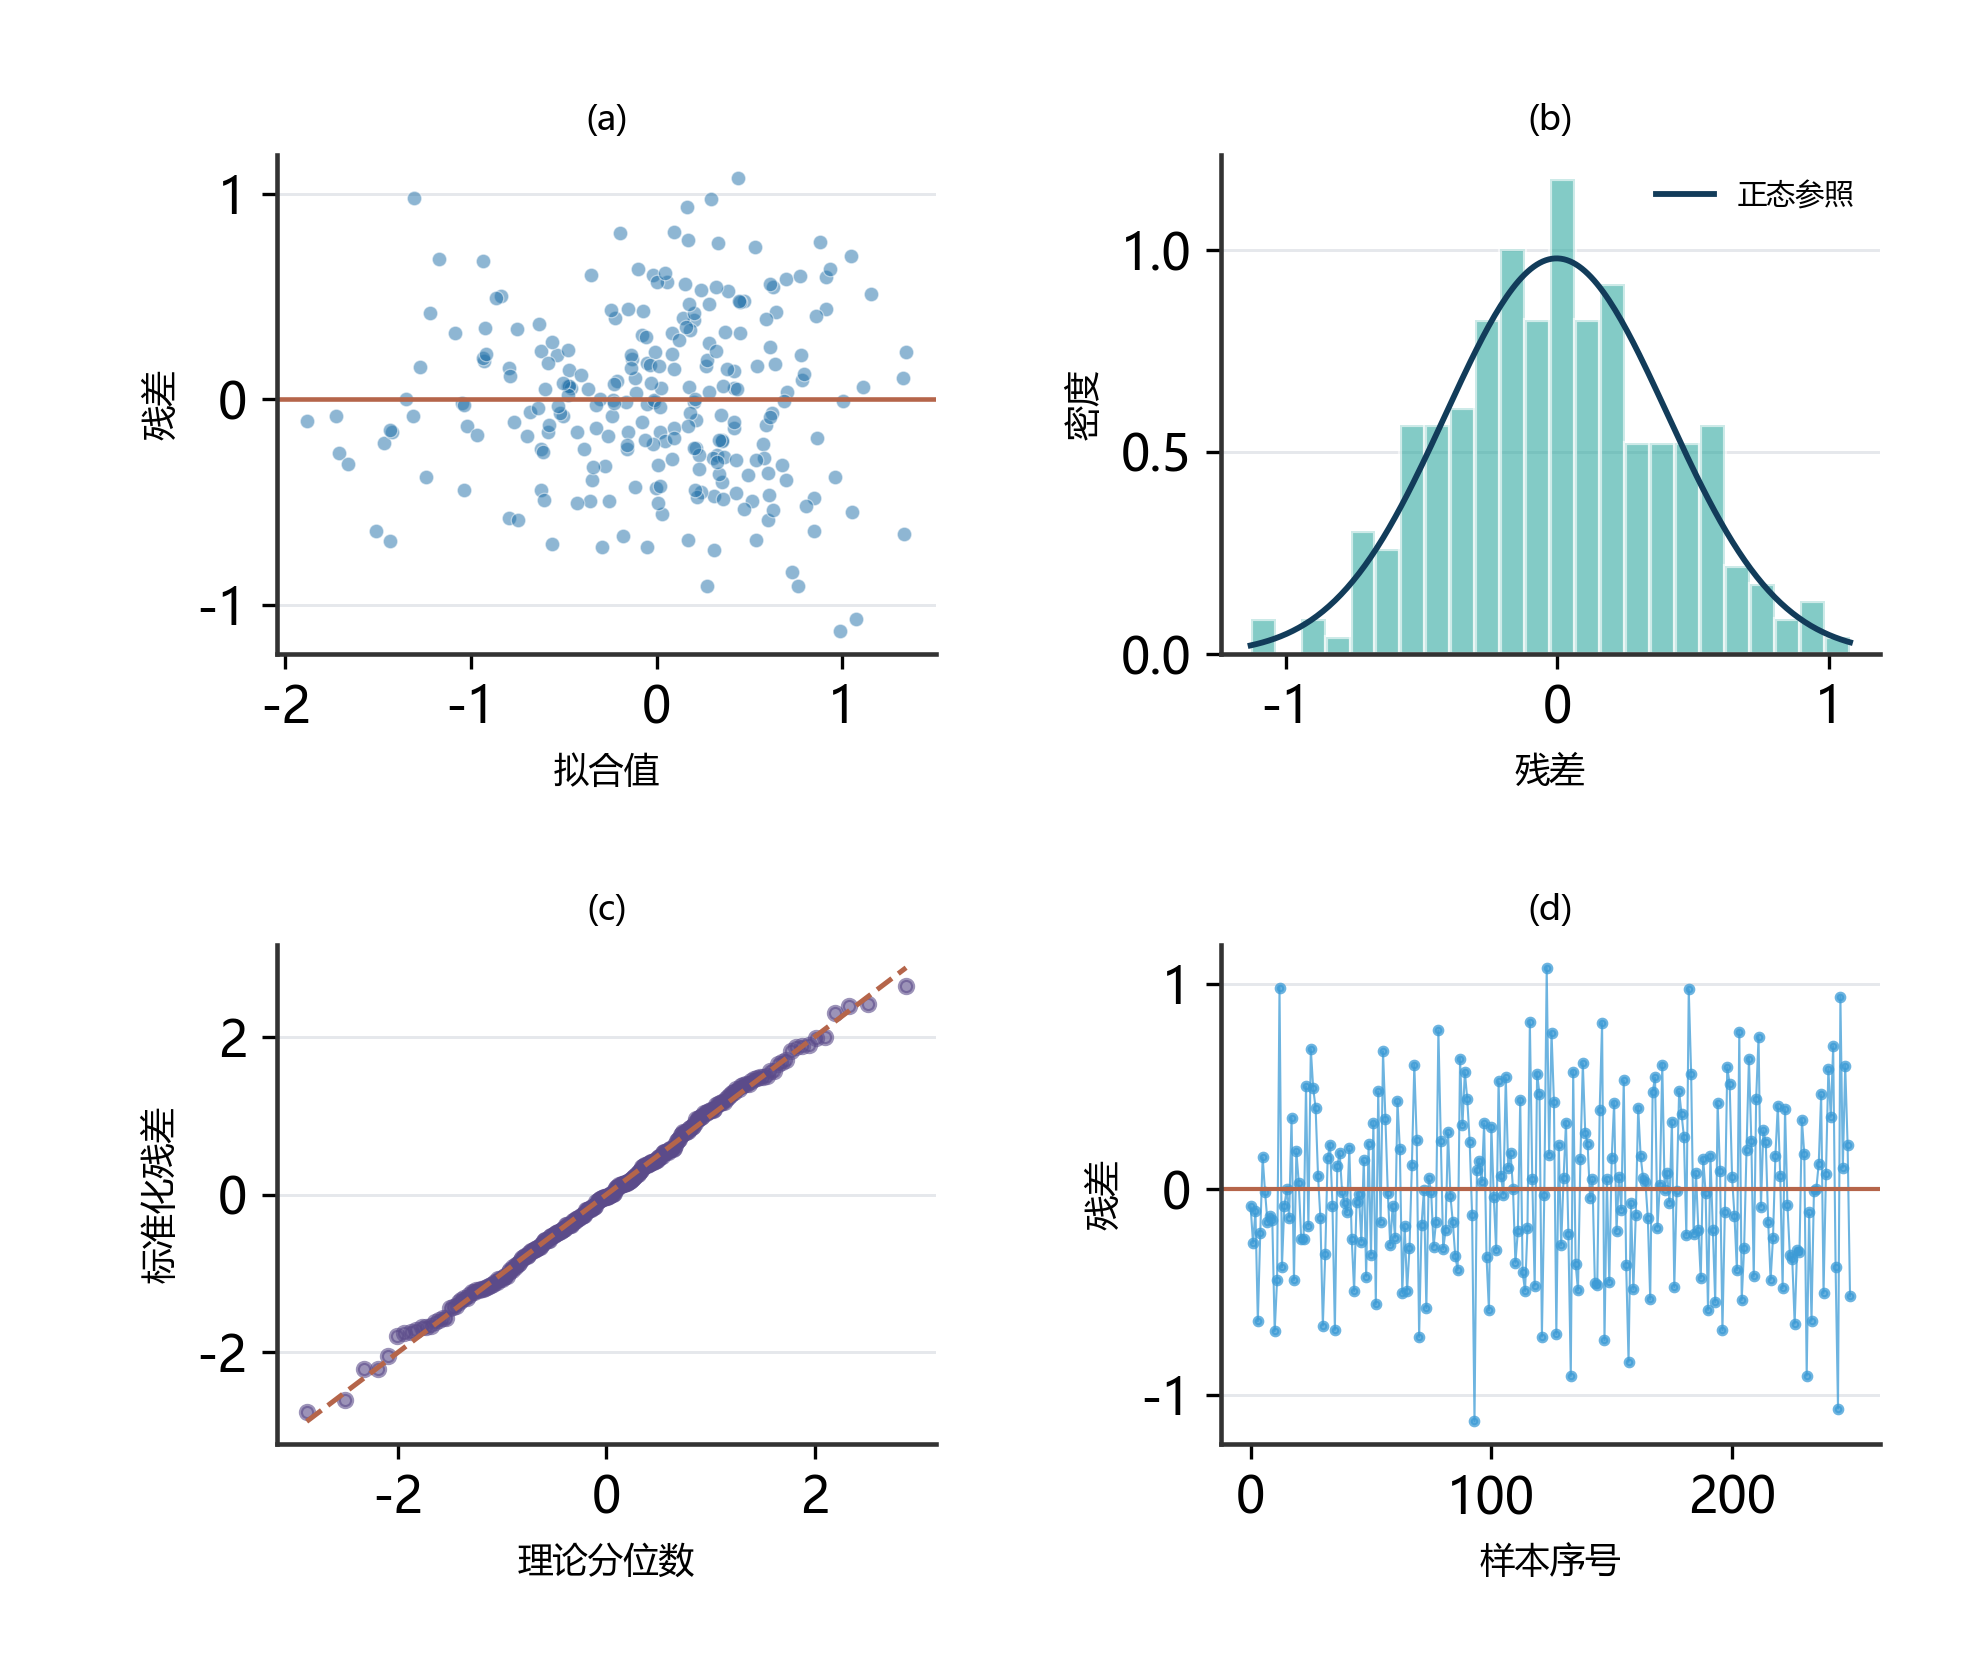
\includegraphics[width=0.62\textwidth]{figures/fig_q1_residual.png}
\caption{alcohol 项的残差四项诊断：残差散点、Q--Q 图、分布直方图与残差序列}
\label{fig:q1res}
\end{figure}

但这套诊断只在可预测的项上成立。推广到全部 50 项，只有 7 项的残差通过正态性检验，其 $p>0.05$；另有 26 项的偏度绝对值超过 1，全表共 189 个样本的标准化残差超过 3 倍标准差。原因与地板效应占比一致：当某一项有 40\% 以上的样本压在最低值时，残差必然是单侧长尾的。

\subsection{结果分析：失效原因与外部效度}

失效原因可以查清。图~\ref{fig:q1floor} 把地板效应占比与 $R^2$ 画在一起，两者的 Spearman 秩相关为 $-0.4009$，明显强于 Pearson 的 $-0.1158$，说明起作用的是单调关系而非线性关系：某项的左尾样本占比越高，模型越难学。这也是把 0.30 定为两段式触发阈值的依据。需要说明的是，两段式组的平均 $R^2$ 为 0.1823，低于非两段式组的 0.2310，即两段式并没有提升精度；它的价值在于把“是否感知”与“感知多强”分开表述，使 acetic、lactic 这类高地板效应占比项的结果可以解释。

\begin{figure}[htbp]
\centering
\begin{subfigure}[t]{0.48\textwidth}
\centering
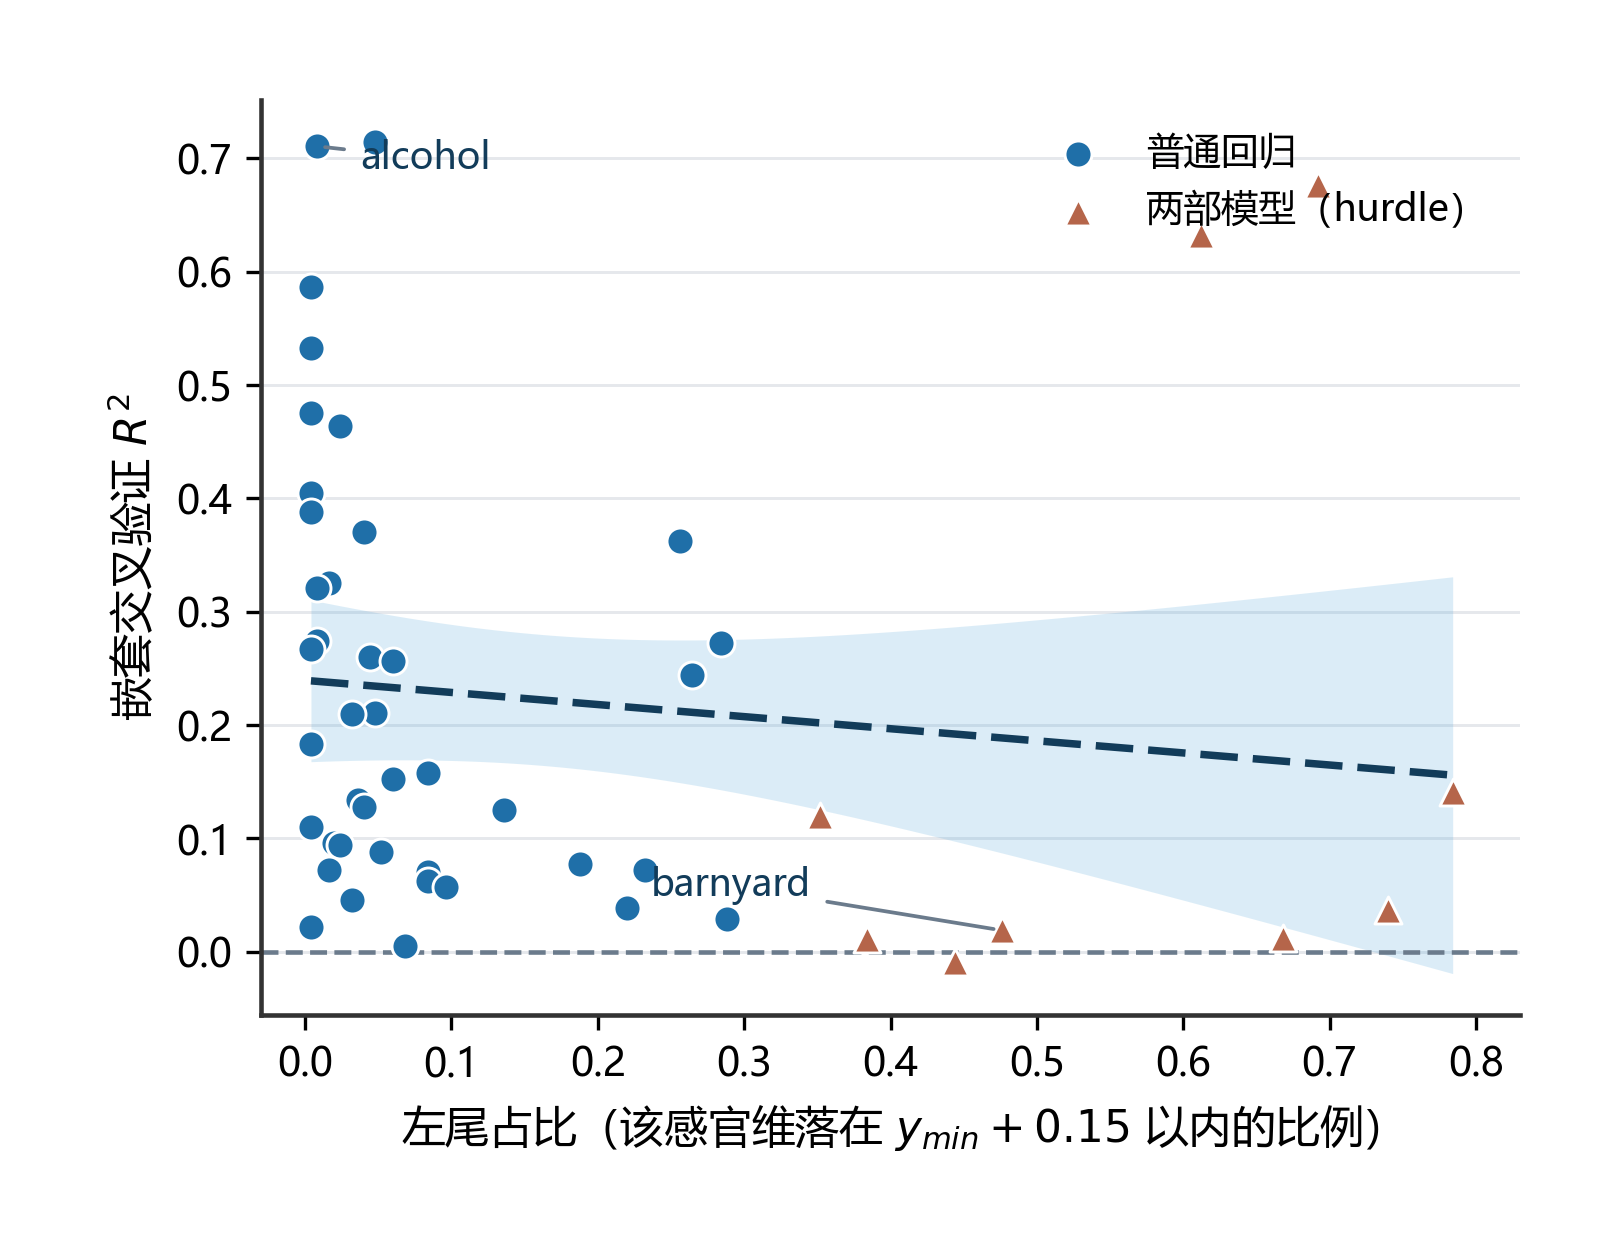
\includegraphics[width=\linewidth]{figures/fig_q1_floor_vs_r2.png}
\caption{左尾占比与 $R^2$ 的单调关系：左尾样本占比越高，模型越难学}
\label{fig:q1floor}
\end{subfigure}
\hfill
\begin{subfigure}[t]{0.48\textwidth}
\centering
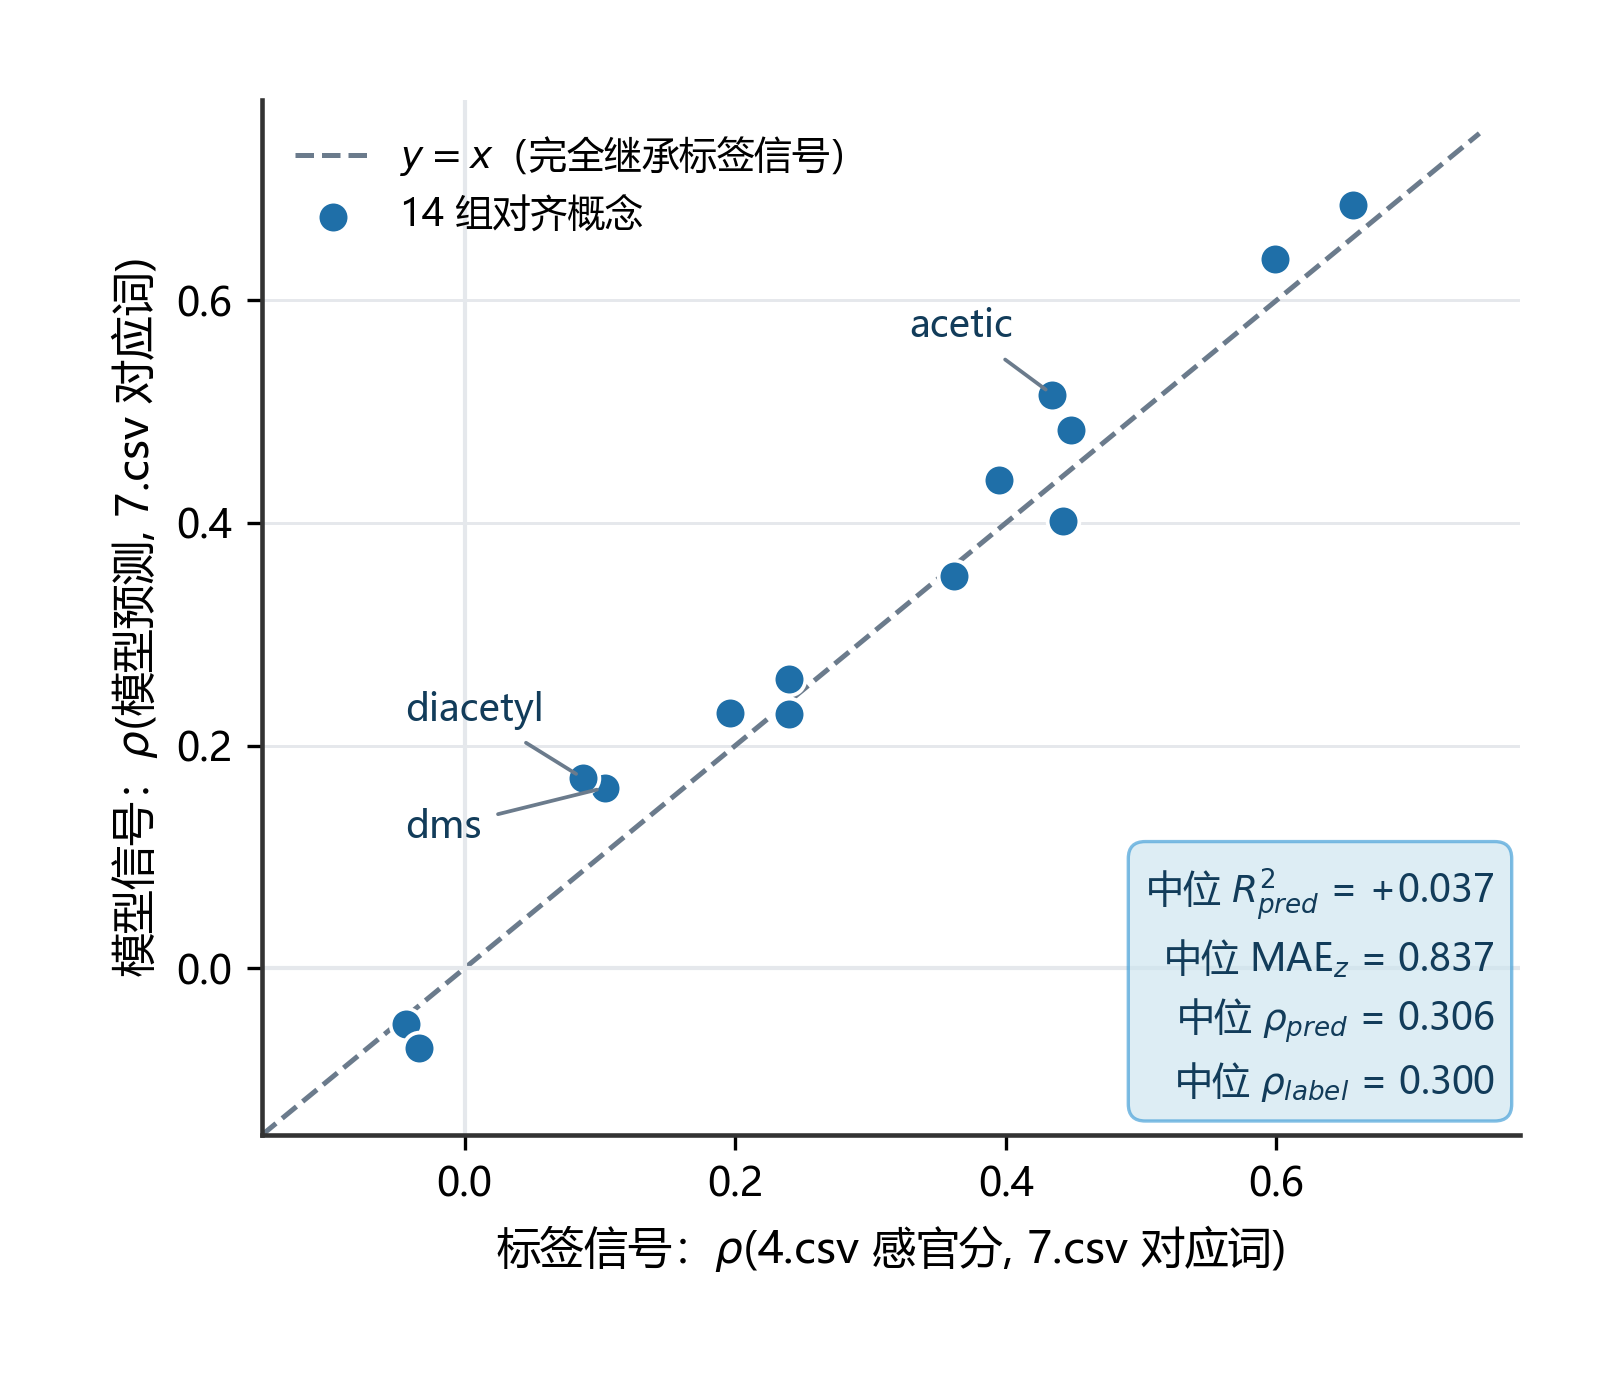
\includegraphics[width=\linewidth]{figures/fig_q1_external.png}
\caption{外部效度：模型预测与原始标签对附件7 的解释力对比，两线贴近对角线说明二者信息量相当}
\label{fig:q1ext}
\end{subfigure}
\caption{失效诊断与外部效度。左图为地板效应占比与 $R^2$ 的单调关系，是 0.30 触发阈值的依据；右图为模型预测与原始标签对附件7 的解释力对比}
\end{figure}

最后做外部效度检验。附件7 是一套独立的论坛评论描述符，与附件4 不同源。做法是在全部 250 个样本上用岭回归拟合"化学谱→附件4 单项"，再把这套拟合值与该单项在附件7 的对应词算秩相关，中位 0.3062；附件4 原始标签与附件7 的相关中位为 0.3005，两者几乎相同，见图~\ref{fig:q1ext}。

这一步用的是\textbf{全样本拟合}而非折外预测，因此这两个数应读作外部关联的\emph{上界}：它回答的是"化学谱能不能解释与论坛评论同向的感官差异"，不回答"模型泛化到新样本时还能不能"。之所以不换成折外预测，是因为附件7 与附件4 的语义对应只覆盖 14 个感官项（50 项中其余 36 项在论坛描述符里没有对应词），样本量不足以支撑逐项的折外检验。这说明模型确实学到了与真实品饮感受相关的信号，但没有比原始标签提供更多信息。跨附件 $R^2$ 中位仅 0.0372、z 尺度平均绝对误差 0.8368，也印证两套标签体系不能互相替代——附件7 只能作参照，不能当第二份训练数据。



\subsection{0--6 分级映射}

题面要求给出 0--6 分的评分。6.1 节已经说明附件4 只有中心化连续值，仿射搜索的残差落在 0.11 到 0.15、落不到整数格点，原始整数分不能精确还原。本节用\emph{先验分位映射}把连续预测转成等级：先在每一项内把强度换成百分位秩，再按给定的等级比例把秩切成 7 档
\begin{equation}
  g_{is}=\sum_{k=0}^{5}\mathbb{I}\left(r_{is}>C_{s,k}\right),\qquad
  C_{s,k}=\sum_{l=0}^{k}p_l,\qquad
  r_{is}=\frac{\operatorname{rank}\left(y_{is}\right)}{n},
\end{equation}
其中 $r_{is}\in(0,1]$ 为第 $s$ 项内第 $i$ 个样本的百分位秩，$p=(p_0,\dots,p_6)$ 为各等级的预期比例，$C_{s,k}$ 为累积切点。这里有一个必须讲清的度量口径。附件4 的原始 0--6 分值不可反解，因此不存在"真值切点"可以直接套到预测上——真值本身也只是一列连续强度。本文的做法是把真值与预测\emph{各自}映射到同一目标边际（即 $p$ 规定的等级比例），再比较两边落在同档的比例。这样度量的是\textbf{同一目标边际下的档位一致性}，衡量排序与分档的吻合程度，不是对面板真值的绝对分级精度。

由此有两点限制必须在读表~\ref{tab:q1grade} 时记住。其一，两条被映射后的分布在按构造上具有相同的等级比例，因此两者的总变差距离恒为 0，这个数不能作为"拟合好"的证据，本文也不报它。其二，分位映射会把预测的边际强行对齐到先验，若先验本身偏离真实边际，kappa 会同时偏高或偏低——这正是表~\ref{tab:q1grade} 要给出四组先验对照的原因：四组的 kappa 中位落在 0.3400 到 0.3812 之间、极差 0.041，说明结论对先验不敏感，但绝对水平依赖先验选择。

等级比例 $p$ 没法从数据反推。附件4 已按品评员做过 z-score 并按啤酒平均，这一步把原始 7 点量表上的厚零结构抹平了：实测每一列的最高频取值只占 1.8\%、恰等于列最小值的样本只占 0.88\%，因此“大量样品取最低档”这一结构\emph{在这份中心化数据上观察不到}。$p$ 只能取自 7 点感官量表的经验分布。

需要说明一处：表~\ref{tab:q1grade} 里零膨胀先验的 kappa（0.3400）并非四组中最高（均匀先验 0.3812、等频映射 0.3770、轻度零膨胀 0.3599）。本文仍以零膨胀为主方案，理由不是 kappa 最高，而是零膨胀的形状与 7 点量表的原始评分结构一致——感官打分中最低两档通常占比最大，这是量表本身的特性，不因本文数据经过中心化而改变；其余三组作为敏感性对照，用于界定“换先验会改变多少”。换言之，主方案按\emph{先验合理性}选定，kappa 的四组差异（极差 0.041）只用于说明该选择对结论的影响幅度，不用于反向挑选最高分。主方案取零膨胀分布 $p=(0.50,\allowbreak 0.18,\allowbreak 0.12,\allowbreak 0.09,\allowbreak 0.06,\allowbreak 0.035,\allowbreak 0.015)$；另设三组对照：均匀分布($p$ 全为 $1/7$)、轻度零膨胀 $p=(0.35,\allowbreak 0.20,\allowbreak 0.16,\allowbreak 0.13,\allowbreak 0.09,\allowbreak 0.05,\allowbreak 0.02)$、等频映射($p$ 全为 $1/7$ 且切点严格取该列的 6 个等分位点)。

\begin{table}[htbp]
\centering
\footnotesize
\caption{0--6 分数映射的四组设定与取整对照，取 50 项中位值}
\label{tab:q1grade}
\footnotesize
\setlength{\tabcolsep}{4.5pt}
\begin{tabular*}{\textwidth}{@{\extracolsep{\fill}}lccccc@{}}
\toprule
\textbf{映射方案} & \textbf{kappa} & \textbf{同档率} & \textbf{$\pm1$ 档} & \textbf{等级 MAE} & \textbf{压 0 占比} \\
\midrule
零膨胀分布（本文） & 0.3400 & 0.390 & 0.672 & 1.208 & -- \\
均匀分布 & 0.3812 & 0.216 & 0.538 & 1.690 & -- \\
轻度零膨胀 & 0.3599 & 0.298 & 0.630 & 1.356 & -- \\
等频映射 & 0.3770 & 0.216 & 0.530 & 1.694 & -- \\
\midrule
平移后直接取整（反例） & 0.1244 & 0.406 & -- & -- & 53.2\% \\
\bottomrule
\end{tabular*}
\end{table}

表~\ref{tab:q1grade} 的第一组结论是等级比例的影响有限：四组设定的加权 kappa 中位落在 0.3400 到 0.3812 之间，极差 0.041。换言之，改变等级比例只改变绝对水平，不改变哪些项可预测。这一点排除了“结论由比例挑选出来”的疑虑。

四组设定之间仍有一处实质差异，即精确同档率：零膨胀分布 0.376，其余三组只有 0.21 左右。原因在于附件4 的标签集中在中低档，而零膨胀比例把切点推向低档，预测与标签在低档更容易重合。这不等于精度更高——同档率只统计“落在同一档”的比例，不区分相邻档的错位，而 kappa 用二次权重、跨档越远罚得越重，因此本文以 kappa 为主要依据。

表~\ref{tab:q1grade} 最后一行是关键对照。若按“先平移到非负再四舍五入”这种看似自然的做法，中位 53.2\% 的样本被压到 0 分，加权 kappa 掉到 0.1244，与随机分档无异。值得注意的是这一行的精确同档率反而高达 0.406，甚至高于主方案——这正是同档率不能单独使用的证据：预测全部压在最低档，与同样集中于低档的标签大范围重合，同档率被“双方都取 0”抬起来。可见分级映射不是收尾步骤，而是问题一能否成立的前提。

50 项的 kappa 中位 0.3400、34 项超过 0.3、16 项超过 0.5；最优的 lactic 达 0.7414，最差的 overall 仅 0.1531。这与连续域的 $R^2$ 中位 0.1469 是同一件事的两种表述：化学谱对感官的解释力本身有限，分级只是把这种有限性摆到明面上。因此分级结果按项分层使用：kappa 高于 0.5 的可作评分参考，0.3 到 0.5 之间只宜作相对比较，低于 0.3 的不宜单独解读。此外附件4 没有 0--6 真值，本文报告的 kappa 与同档率都是同一映射内的往返一致性，衡量预测分与标签分落在同一档的比例，不是对感官面板真值的绝对精度。这条限制换模型也消除不了，只能如实标注。
